\documentclass[11pt,a4paper]{article}

\usepackage[french]{babel}
\usepackage[T1]{fontenc}
\usepackage[utf8]{inputenc}
\usepackage{lmodern}
\usepackage{microtype}
\usepackage{geometry}
\usepackage{graphicx}
\usepackage{booktabs}
\usepackage{hyperref}
\usepackage{caption}
\usepackage{subcaption}
\usepackage{enumitem}

\geometry{margin=2.5cm}
\hypersetup{colorlinks=true, linkcolor=blue, urlcolor=blue, citecolor=blue}

\title{Application Business Intelligence\\Démissions d'un organisme bancaire}
\author{Mehdi \and Rayane}
\date{\today}

\begin{document}

\maketitle

\begin{abstract}
Ce document présente l'\textbf{exploration}, le \textbf{nettoyage}, la \textbf{concaténation}, le \textbf{recodage}, le \textbf{prétraitement} et le \textbf{découpage} train\,/\,validation\,/\,test (\texttt{decoupage.py}). Objectif : \textbf{classification} du risque de démission. Sorties : \texttt{exploration/}, \texttt{nettoyage/}, \texttt{concatenation/}, \texttt{recodage/}, \texttt{pretraitement/}, \texttt{decoupage/}.
\end{abstract}

\tableofcontents
\newpage

\section{Contexte et objectifs}

L'objectif du projet est d'identifier des profils de sociétaires à risque de démission, puis de construire ultérieurement un score d'attrition et d'en analyser l'explicabilité. La phase documentée ici se limite à l'\textbf{exploration descriptive et associative} des données historiques (\texttt{table1}) et de l'échantillon mélangé actuels/passés (\texttt{table2}), conformément au cahier des charges du module.

\section{Exploration}

\subsection{Données et principes}

\begin{itemize}[leftmargin=*]
  \item \textbf{Fichiers} : \texttt{data/table1.csv} (démissionnaires, 1999--2006) et \texttt{data/table2.csv} (échantillon aléatoire incluant démissionnaires et non-démissionnaires).
  \item \textbf{Aucun nettoyage} : les valeurs aberrantes ou sentinelle (ex.\ dates \texttt{0000-00-00}, \texttt{31/12/1900}) sont conservées telles quelles pour ne pas biaiser cette étape par des choix implicites.
  \item \textbf{Exclusion} : la colonne \texttt{ID} est exclue des analyses (pas de lien entre les deux tables).
  \item \textbf{Typage} : classification \emph{quantitatif} vs \emph{qualitatif} selon les types lus par \texttt{pandas} (entiers et flottants = quantitatifs ; texte = qualitatifs).
\end{itemize}

\subsection{Outils mis en œuvre}

L'exploration est automatisée par le script \texttt{exploration.py} à la racine du projet, qui s'appuie sur deux bibliothèques internes :

\begin{description}
  \item[\texttt{analyse}] Résumés univariés (moyenne, médiane, écart-type, quartiles, mode\ldots) ; bivarié quanti--quanti (Pearson, Spearman, Kendall et tests associés) ; quali--quali ($\chi^2$, degrés de liberté, Cramér $V$) ; quanti--quali (Kruskal--Wallis, ANOVA à un facteur, $\varepsilon^2$ pour Kruskal--Wallis).
  \item[\texttt{graphique}] Histogrammes, diagrammes en barres, nuages de points, heatmaps de corrélation, boîtes à moustaches, barres de contingence.
\end{description}

Les dépendances sont listées dans \texttt{requirements.txt} (\texttt{pandas}, \texttt{numpy}, \texttt{scipy}, \texttt{matplotlib}, \texttt{seaborn}).

\subsection{Organisation des sorties}

Pour chaque table, les résultats sont séparés en deux sous-dossiers :

\begin{center}
\texttt{exploration/table1/univariate/} \quad ; \quad \texttt{exploration/table1/bivariate/} \\
\texttt{exploration/table2/univariate/} \quad ; \quad \texttt{exploration/table2/bivariate/}
\end{center}

\noindent On y trouve des fichiers CSV récapitulatifs (\texttt{resume\_univarie\_*.csv}, \texttt{resume\_bivarie\_*.csv}) et l'ensemble des graphiques générés (toutes les paires de colonnes hors \texttt{ID} pour le bivarié, plus des heatmaps Pearson et Spearman sur les variables numériques).

\subsection{Résultats illustrés (sélection)}

\subsubsection{Univarié}

La figure~\ref{fig:mtrev} montre la distribution des revenus dans \texttt{table2} : forte asymétrie (nombreux zéros, queue droite). La figure~\ref{fig:agead} présente l'âge à l'adhésion dans \texttt{table1}.

\begin{figure}[htbp]
  \centering
  
\includegraphics[width=0.75\textwidth]{img/MTREV_histogramme.png}
  \caption{\texttt{table2} --- distribution de \texttt{MTREV} (montant des revenus).}
  \label{fig:mtrev}
\end{figure}

\begin{figure}[htbp]
  \centering
  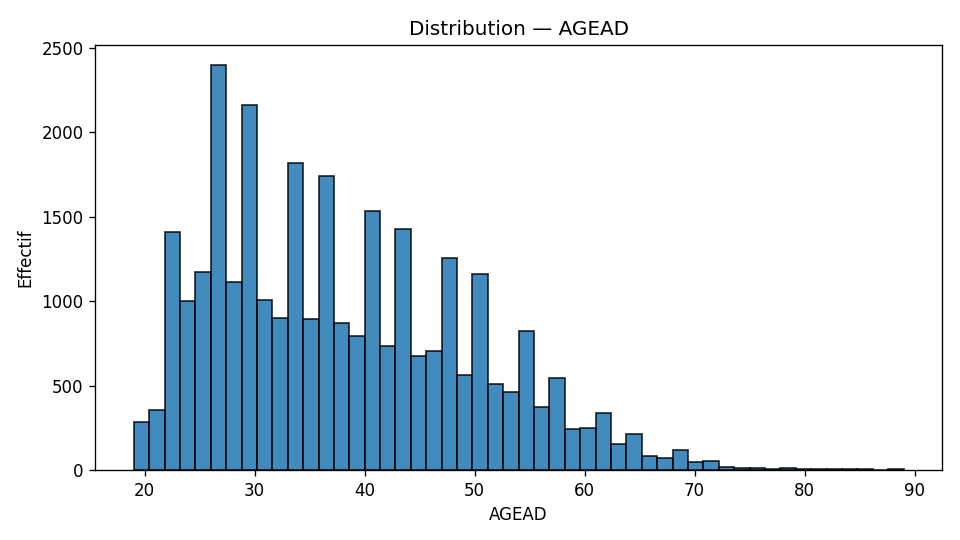
\includegraphics[width=0.75\textwidth]{img/AGEAD_histogramme.png}
  \caption{\texttt{table1} --- distribution de \texttt{AGEAD} (âge à l'adhésion).}
  \label{fig:agead}
\end{figure}

\subsubsection{Corrélations entre variables numériques}

Les heatmaps (Pearson) synthétisent les associations linéaires entre toutes les colonnes numériques d'une même table (figures~\ref{fig:heat1} et~\ref{fig:heat2}).

\begin{figure}[htbp]
  \centering
  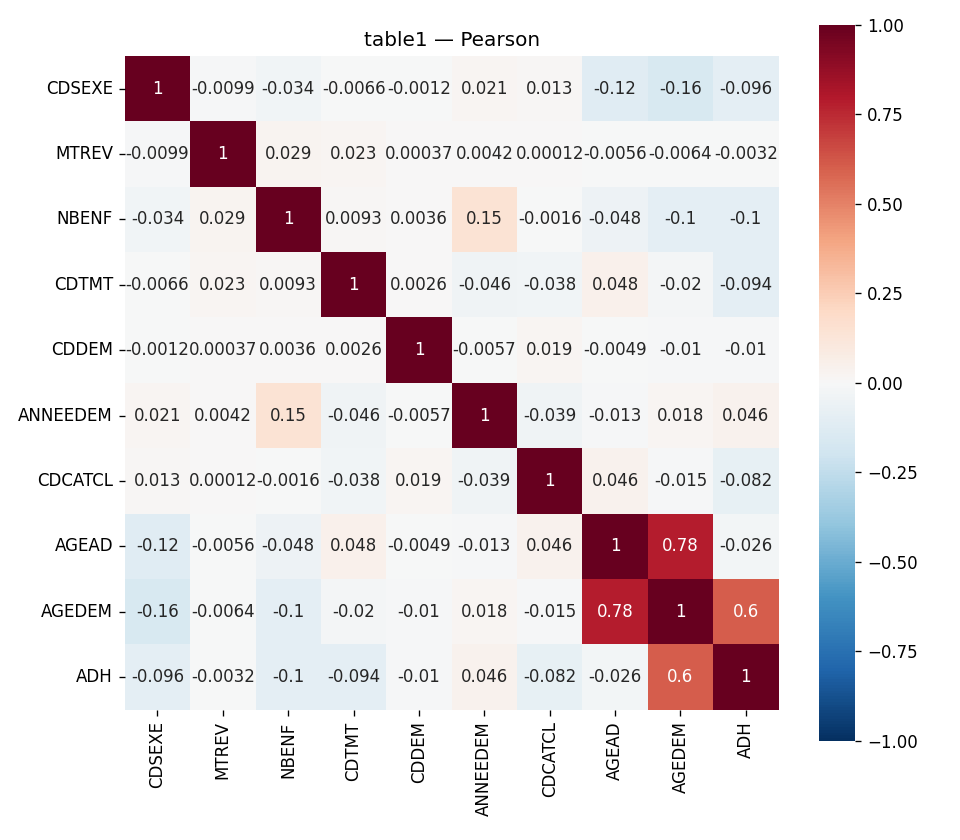
\includegraphics[width=0.92\textwidth]{img/heatmap_pearson_table1.png}
  \caption{\texttt{table1} --- matrice de corrélations de Pearson entre variables quantitatives.}
  \label{fig:heat1}
\end{figure}

\begin{figure}[htbp]
  \centering
  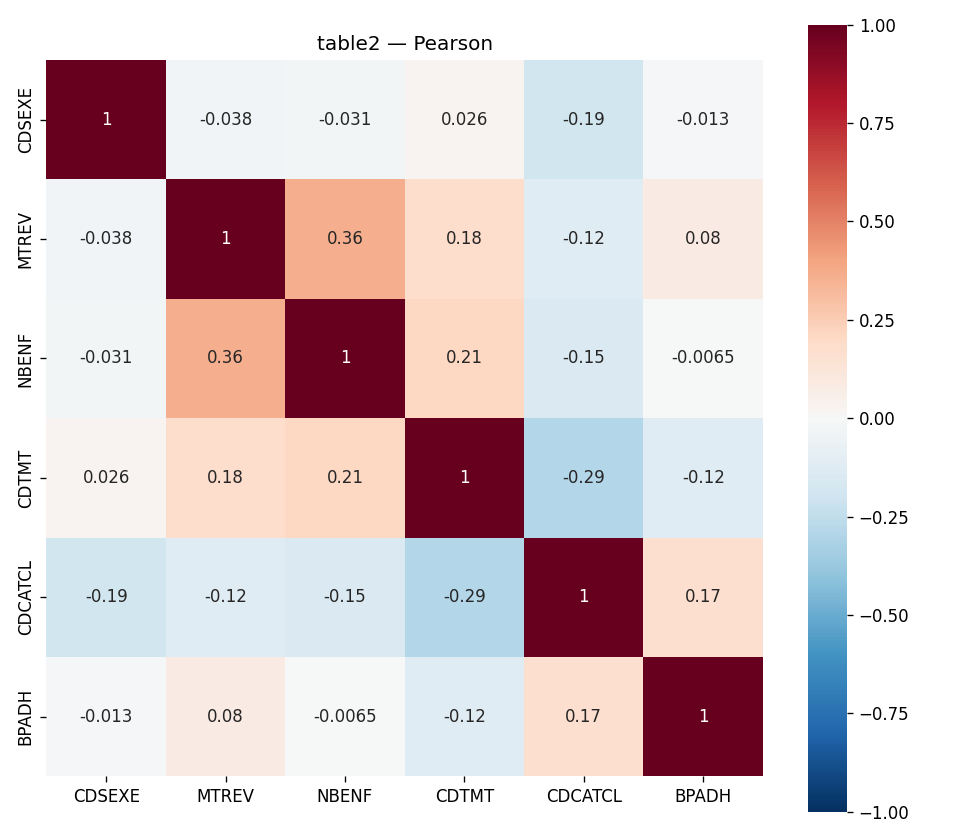
\includegraphics[width=0.85\textwidth]{img/heatmap_pearson_table2.png}
  \caption{\texttt{table2} --- matrice de corrélations de Pearson entre variables quantitatives.}
  \label{fig:heat2}
\end{figure}

\subsubsection{Associations quanti--quanti (nuages de points)}

La figure~\ref{fig:age} met en évidence une corrélation forte entre âge à l'adhésion et âge à la démission dans \texttt{table1}. La figure~\ref{fig:adh} relie l'ancienneté (\texttt{ADH}) à l'âge à la démission.

\begin{figure}[htbp]
  \centering
  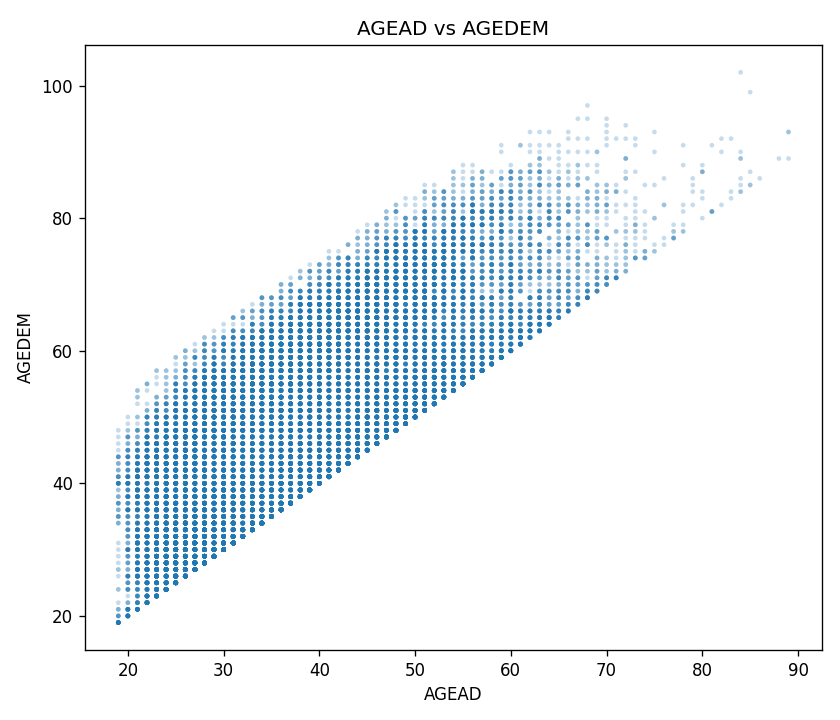
\includegraphics[width=0.75\textwidth]{img/AGEAD__AGEDEM_nuage.png}
  \caption{\texttt{table1} --- \texttt{AGEAD} vs \texttt{AGEDEM} (nuage de points).}
  \label{fig:age}
\end{figure}

\begin{figure}[htbp]
  \centering
  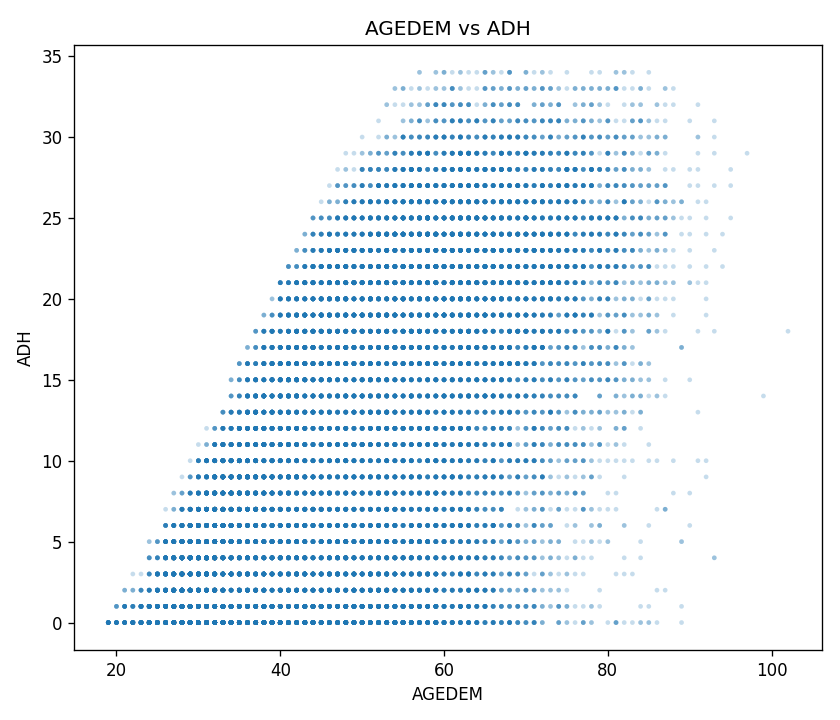
\includegraphics[width=0.75\textwidth]{img/ADH__AGEDEM_nuage.png}
  \caption{\texttt{table1} --- \texttt{ADH} (durée d'adhésion) vs \texttt{AGEDEM}.}
  \label{fig:adh}
\end{figure}

Dans \texttt{table2}, le lien entre \texttt{MTREV} et \texttt{NBENF} est illustré figure~\ref{fig:mtrev_nb}.

\begin{figure}[htbp]
  \centering
  
\includegraphics[width=0.75\textwidth]{img/MTREV__NBENF_nuage.png}
  \caption{\texttt{table2} --- \texttt{MTREV} vs \texttt{NBENF}.}
  \label{fig:mtrev_nb}
\end{figure}

\subsubsection{Quanti--quali : boîtes à moustaches}

La figure~\ref{fig:boites} compare la distribution de \texttt{AGEAD} selon les modalités de \texttt{RANGAGEAD} (tranche d'âge à l'adhésion) : la redondance informationnelle entre âge numérique et tranche est visible.

\begin{figure}[htbp]
  \centering
  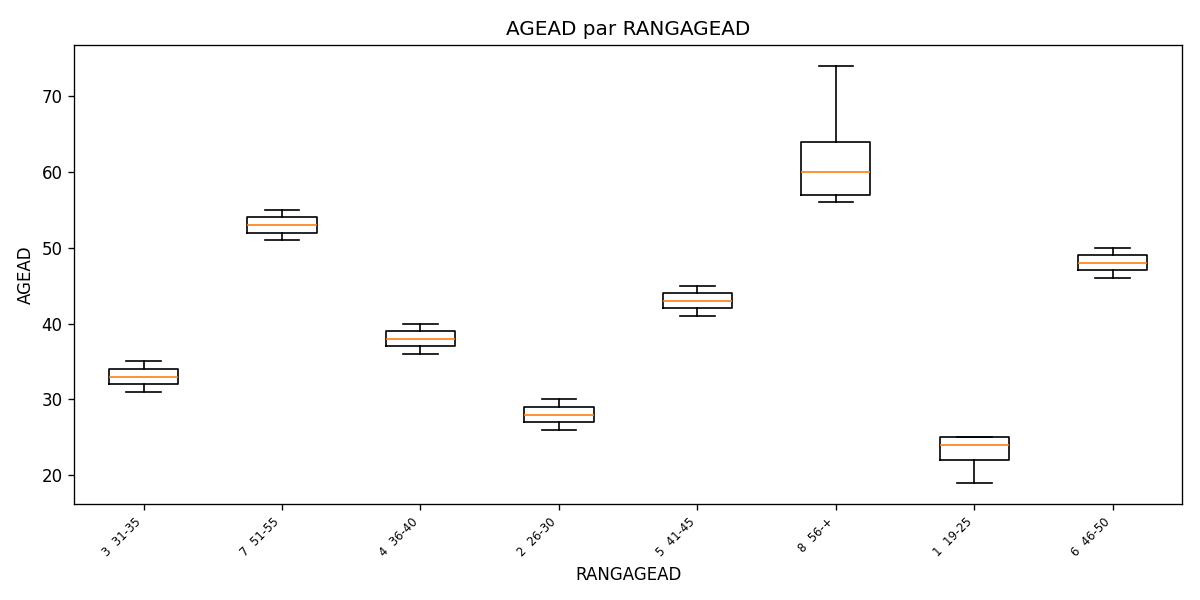
\includegraphics[width=0.85\textwidth]{img/AGEAD__RANGAGEAD_boites.png}
  \caption{\texttt{table1} --- \texttt{AGEAD} par modalité de \texttt{RANGAGEAD}.}
  \label{fig:boites}
\end{figure}

\subsection{Synthèse et limites de cette phase}

\begin{itemize}[leftmargin=*]
  \item Les tests sont nombreux (toutes les paires) : les $p$-valeurs doivent être interprétées avec prudence (multiplicité) ; les tailles d'effet (coefficients de corrélation, Cramér $V$, $\varepsilon^2$) complètent la lecture.
  \item Les variables à très nombreuses modalités (dates en chaîne de caractères) produisent des $\chi^2$ élevés et des graphiques de contingence peu lisibles : elles seront à traiter ultérieurement (agrégation, features temporelles) hors périmètre « exploration brute ».
  \item La suite du projet (modélisation supervisée, score, explicabilité) s'appuiera sur une définition explicite de la cible démission à partir de \texttt{table2} (\texttt{DTDEM}, \texttt{CDMOTDEM}, etc.).
\end{itemize}

\section{Nettoyage}

L'objectif final du projet est d'\textbf{identifier les sociétaires à risque de départ}, ce qui sera réalisé ultérieurement par des \textbf{méthodes de classification} supervisées. La préparation des données n'est pas une simple suppression de lignes : il s'agit de rendre les variables \textbf{cohérentes}, \textbf{interprétables} et \textbf{exploitables} par un modèle, tout en documentant les choix. Les constats ci-dessous s'appuient sur le script \texttt{nettoyage.py} (sorties dans \texttt{nettoyage/}) et sur l'exploration précédente.

\subsection{Ces données nécessitent-elles un nettoyage ?}

\textbf{Constat.} Les fichiers mélangent \textbf{dates en texte}, \textbf{codes sentinelles} explicites dans l'énoncé (\texttt{0000-00-00} pour une naissance inconnue, \texttt{31/12/1900} pour un non-démissionnaire dans \texttt{table2}), des \textbf{entiers} parfois catégoriels, et des distributions très \textbf{asymétriques} (ex.\ \texttt{MTREV}, figure~\ref{fig:mtrev}).

\textbf{Idée.} Le «~nettoyage~» recouvre ici la \textbf{préparation} : recodage des sentinelles, parsing ou dérivation de features à partir des dates, encodage des modalités, transformations éventuelles des variables continues à queue lourde.

\textbf{Solution.} Mettre en place une chaîne de traitements \textbf{traçable} (reproductible) avant l'apprentissage : définition de la variable cible (démission oui/non), traitement des manquants structurels, sélection ou dérivation de variables pour limiter la redondance.

\textbf{Explication.} Sans préparation, un classifieur mélange absences d'information codées et valeurs réelles, et peut être dominé par quelques modalités extrêmes ou par des doublons informationnels.

\subsection{Faut-il écarter certaines instances qui ne sont pas liées au problème ?}

\textbf{Constat.} Le script \texttt{nettoyage.py} ne détecte \textbf{aucune ligne entièrement vide} sur \texttt{table2} (15\,022 lignes). Les valeurs atypiques repérées relèvent surtout de \textbf{codes métier}, pas d'enregistrements invalides. Par ailleurs, \texttt{table1} ne contient que des \textbf{démissionnaires} et \texttt{table2} un mélange : ce sont des \textbf{populations différentes}.

\textbf{Idée.} «~Non lié au problème~» doit être défini par le \textbf{périmètre métier} (qui prédire ? à quelle date d'extraction ?), pas seulement par un critère statistique automatique.

\textbf{Solution.} Ne pas supprimer massivement les lignes portant des sentinelles ; éventuellement \textbf{restreindre la population} (ex.\ critères d'éligibilité) uniquement si le cahier des charges le fixe explicitement. Ne pas fusionner naïvement \texttt{table1} et \texttt{table2} pour un score sur sociétaires «~actuels~» sans stratégie d'échantillonnage.

\textbf{Explication.} Exclure des individus sans justification métier \textbf{biaise} l'inférence ; les sentinelles se \textbf{recodent} (manquant, indicateur, modalité dédiée).

\subsection{Sur quoi se base-t-on pour prendre cette décision ?}

\textbf{Constat.} Plus sources se combinent : dictionnaire des variables, fichiers \texttt{manquants\_table*.csv}, \texttt{sentinelles\_table*.json}, \texttt{redondances.csv}, \texttt{typologie\_attributs.csv}, résultats de l'exploration (corrélations, Cramér~$V$), et contraintes du futur modèle (ex.\ arbres vs régression).

\textbf{Idée.} Décision \textbf{data + objectif + modèle} : une règle purement automatique (seuil IQR, etc.) ne suffit pas sans validation métier.

\textbf{Solution.} Documenter chaque règle (recodage, exclusion éventuelle, transformation) dans le rapport de préparation et, plus tard, dans la validation du modèle.

\textbf{Explication.} La traçabilité est indispensable pour la \textbf{reproductibilité} et l'\textbf{explicabilité} attendues en BI.

\subsection{Y a-t-il des valeurs manquantes ?}

\textbf{Constat.} \textbf{Table1} : seuls des manquants \texttt{pandas} sur \textbf{\texttt{RANGADH}} --- 2\,584 cas (8{,}52\,\% du fichier). \textbf{Table2} : \textbf{\texttt{CDMOTDEM}} compte 14\,195 valeurs manquantes (94{,}49\,\%) ; les autres colonnes n'ont pas de NaN dans l'import brut.

\textbf{Idée.} Le volume élevé sur \texttt{CDMOTDEM} est \textbf{structurel} : le motif de démission n'existe que pour les démissions déclarées.

\textbf{Solution.} Pour \texttt{RANGADH} : imputation, modalité «~inconnu~», ou modèle gérant le NA. Pour \texttt{CDMOTDEM} : l'intégrer comme \textbf{non applicable} hors démission ; la cible de classification reposera plutôt sur \texttt{DTDEM} / absence de motif selon la définition opérationnelle de la démission.

\textbf{Explication.} Un taux de manquants élevé n'indique pas toujours une «~mauvaise qualité globale~» : il peut refléter la \textbf{sémantique} de la variable.

\subsection{Y a-t-il des valeurs aberrantes ?}

\textbf{Constat.} Deux types coexistent. (1) \textbf{Sentinelles} documentées : \texttt{DTNAIS}~=~\texttt{0000-00-00} (164 lignes dans \texttt{table2}) ; \texttt{DTDEM}~=~\texttt{31/12/1900} pour marquer les \textbf{non-démissionnaires} (14\,474 lignes). (2) \textbf{Extrêmes numériques} : par exemple \texttt{MTREV} jusqu'à 1\,524\,490 (table1) et 38\,413 (table2) ; la règle IQR (fichiers \texttt{outliers\_iqr\_*.csv}) classe une part notable de valeurs comme «~hors boîte~» pour \texttt{MTREV} et \texttt{NBENF}, avec prudence pour les variables à masse en zéro.

\textbf{Idée.} Distinguer \textbf{code métier} (à recoder) et \textbf{valeur extrême plausible} (revenu élevé, famille nombreuse).

\textbf{Solution.} Recoder les sentinelles ; pour les continuums, envisager \textbf{log(MTREV+1)}, winsorisation, ou modèles peu sensibles aux queues (arbres) sans suppression systématique des extrêmes.

\textbf{Explication.} Supprimer agressivement les gros revenus peut \textbf{casser} la représentation des profils à risque réels.

\subsection{Y a-t-il des attributs redondants ?}

\textbf{Constat.} L'exploration montre une forte dépendance entre \textbf{âges numériques} (\texttt{AGEAD}, \texttt{AGEDEM}) et les \textbf{tranches} associées (\texttt{RANGAGEAD}, \texttt{RANGAGEDEM}), entre \textbf{\texttt{ADH}} et \textbf{\texttt{RANGADH}}, et une information temporelle dupliquée entre \textbf{\texttt{ANNEEDEM}}, \textbf{\texttt{DTDEM}} et \textbf{\texttt{RANGDEM}} (voir aussi figure~\ref{fig:boites}).

\textbf{Idée.} La redondance peut \textbf{gonfler} la variance des estimateurs ou favoriser le sur-ajustement selon le modèle.

\textbf{Solution.} Ne conserver qu'\textbf{une représentation par famille} (âge continu \emph{ou} tranche ; une échelle de temps cohérente pour la démission).

\textbf{Explication.} Mieux vaut une seule variable bien définie que trois colinéaires.

\subsection{Y a-t-il des attributs superflus ?}

\textbf{Constat.} L'identifiant \texttt{ID} n'apporte pas d'information prédictive. Le champ \textbf{\texttt{BPADH}} reste \textbf{non documenté} dans l'énoncé. Sur \texttt{table1}, le code \textbf{\texttt{CDDEM}} est \textbf{quasi constant} : la figure~\ref{fig:cddem} montre que l'effectif se concentre sur une seule modalité (valeur 2), ce qui confère une \textbf{variance nulle ou négligeable} à cet attribut pour la discrimination.

\begin{figure}[htbp]
  \centering
  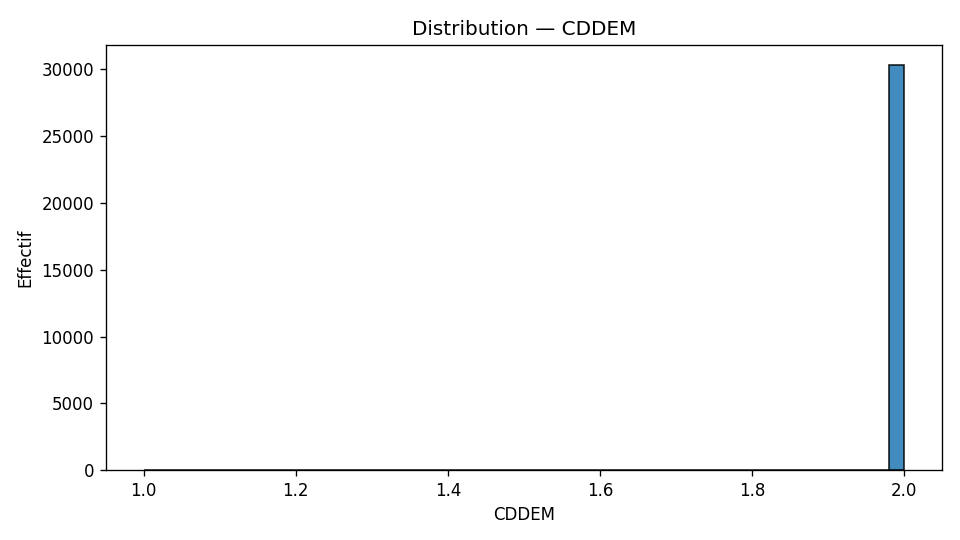
\includegraphics[width=0.72\textwidth]{img/CDDEM_histogramme.png}
  \caption{\texttt{table1} --- distribution de \texttt{CDDEM} : quasi-totalité des observations sur une modalité (variance utile nulle pour un classifieur).}
  \label{fig:cddem}
\end{figure}

\textbf{Idée.} Un prédicteur constant ou quasi constant ne contribue pas au score d'attrition ; il peut être retiré ou ignoré dans la sélection de variables.

\textbf{Solution.} Exclure \texttt{ID} des features ; traiter \texttt{BPADH} après clarification métier ; retirer \texttt{CDDEM} de la liste des prédicteurs pour \texttt{table1} si le constat de quasi-constance se confirme sur le périmètre d'apprentissage.

\textbf{Explication.} Pour la classification, l'objectif est le \textbf{pouvoir discriminant} vis-à-vis de la cible ; les variables sans variation n'en ont pas.

\subsection{Les valeurs numériques correspondent-elles à des grandeurs métriques, ordinales ou catégorielles ?}

\textbf{Constat.} Le typage \texttt{pandas} (entier vs texte) est trompeur : \texttt{CDSEXE}, \texttt{CDTMT}, \texttt{CDCATCL} sont des \textbf{codes catégoriels} ; les \texttt{RANG*} sont des \textbf{ordinaux} (tranches) ; \texttt{AGEAD}, \texttt{AGEDEM}, \texttt{ADH}, \texttt{MTREV} se rapprochent de variables \textbf{métriques} (continues ou comptages).

\textbf{Idée.} Le niveau de mesure guide l'\textbf{encodage} (one-hot, ordinal respectueux, conservation en nombre) et l'interprétation des coefficients ou importances.

\textbf{Solution.} Encoder les nominaux sans ordre naturel ; traiter les ordinaux avec prudence ; ne pas interpréter linéairement un code sexe ou statut comme une «~grandeur~» sans validation.

\textbf{Explication.} Un modèle de classification \textbf{correctement alimenté} évite les faux continuums et améliore la lisibilité des résultats pour la campagne CRM.

\subsection{Comment traiter ces différents problèmes ?}

\textbf{Constat.} Les problèmes se cumulent (manquants, sentinelles, extrêmes, redondance, typage).

\textbf{Idée.} Enchaîner les traitements dans un ordre logique : \textbf{cible} $\rightarrow$ \textbf{recodage} $\rightarrow$ \textbf{sélection/dérivation de variables} $\rightarrow$ \textbf{encodage} $\rightarrow$ \textbf{échantillon d'apprentissement/validation}.

\textbf{Solution.} (1)~Définir la cible binaire (démission) à partir de \texttt{DTDEM} et/ou \texttt{CDMOTDEM}. (2)~Convertir les sentinelles en NA ou indicateurs. (3)~Parser les dates ou en extraire l'ancienneté et l'âge à la date d'extraction (2007). (4)~Réduire la redondance (âge vs tranches). (5)~Transformer ou binariser \texttt{MTREV} si nécessaire. (6)~Imputer ou coder le manquant lorsque pertinent. (7)~Entraîner le classifieur et valider hors échantillon.

\textbf{Explication.} Cette chaîne relie directement le diagnostic (\texttt{nettoyage/}) à l'\textbf{objectif métier} : prioriser les sociétaires à risque pour une action de rétention.

\section{Concaténation}

Les données sont réparties entre \textbf{\texttt{table1}} (démissionnaires historiques, 1999--2006) et \textbf{\texttt{table2}} (échantillon aléatoire de sociétaires actuels et passés). L'énoncé précise que les \textbf{identifiants \texttt{ID} ne correspondent pas} d'une table à l'autre : il n'existe donc \textbf{pas de jointure} possible sur la clé \texttt{ID}. Le script \texttt{concatenation.py} implémente l'\textbf{empilement vertical} sur les colonnes communes, avec sorties dans \texttt{concatenation/} : \texttt{resume\_strategies.json}, \texttt{echantillon\_union\_500lignes.csv}, \texttt{descriptifs\_variables\_communes.csv} (moyennes/médianes indicatives), \texttt{synthese\_concatenation.txt}.

\medskip
\noindent\fbox{\parbox{0.97\linewidth}{
\textbf{À ne pas confondre.} Il y a \textbf{deux questions différentes} :
\begin{enumerate}[leftmargin=*]
  \item \textbf{Concaténer techniquement les fichiers ?} --- \textbf{Oui, c'est fait} : les lignes de \texttt{table1} et \texttt{table2} sont empilées sur les dix colonnes communes, avec \texttt{source} et de nouveaux \texttt{ID} (section~\ref{sec:concat-tech} ci-dessous). Cela produit une \textbf{table unique} exploitable pour exploration ou pour des modèles qui \textbf{utilisent explicitement} l'origine (\texttt{source}) ou une pondération.
  \item \textbf{Sur quelle base entraîner surtout le classifieur churn / non-churn ?} --- Là, on \textbf{recommande de partir de \texttt{table2}} comme \textbf{jeu principal}, parce qu'y coexistent démissionnaires et non-démissionnaires dans \textbf{un même échantillon} ; la cible se déduit de \texttt{DTDEM}. Ce n'est \textbf{pas} dire «~on n'a pas concaténé~» : c'est dire qu'\textbf{entraîner uniquement sur l'union sans précaution} mélange une population (historique \textbf{tous} démissionnaires) avec une autre et \textbf{déforme} la proportion de positifs par rapport à ce qu'on observe dans \texttt{table2}.
\end{enumerate}
}}

\subsection{Faut-il concaténer les tables ?}

\textbf{Constat.} Les deux tables ne décrivent pas la même \textbf{population statistique} : \texttt{table1} ne contient que des \textbf{démissionnaires} ; \texttt{table2} contient à la fois des démissionnaires et des non-démissionnaires (date de démission sentinelle \texttt{31/12/1900}). Les colonnes se \textbf{recouvrent partiellement} : \textbf{dix} attributs communs (\texttt{ID}, \texttt{CDSEXE}, \texttt{MTREV}, \texttt{NBENF}, \texttt{CDSITFAM}, \texttt{DTADH}, \texttt{CDTMT}, \texttt{CDMOTDEM}, \texttt{CDCATCL}, \texttt{DTDEM}), alors que neuf attributs sont propres à \texttt{table1} (âges, tranches, \texttt{ANNEEDEM}, etc.) et deux à \texttt{table2} (\texttt{DTNAIS}, \texttt{BPADH}).

\textbf{Idée.} Concaténer n'est pas une nécessité logique : c'est un choix de \textbf{modélisation}. On peut travailler sur \texttt{table2} seul pour un problème supervisé \textbf{churn / non-churn}, ou fusionner des informations sous conditions strictes.

\textbf{Solution.} Trois approches typiques :
\begin{enumerate}[leftmargin=*]
  \item \textbf{Union verticale} sur les colonnes communes uniquement, avec une variable \texttt{source} $\in$ \{\texttt{table1}, \texttt{table2}\} et un réidentifiant les \texttt{ID} locaux pour éviter les collisions entre fichiers ;
  \item \textbf{\texttt{table2} seul} : base naturelle pour estimer la probabilité de démission observée dans l'échantillon, avec cible dérivée de \texttt{DTDEM} ;
  \item \textbf{Union + label explicite} : étiqueter chaque ligne (ex.\ démission oui/non) en traitant \texttt{table1} comme \textbf{tous positifs} historiques et \texttt{table2} selon la sentinelle --- utile pour diagnostiquer le \textbf{déséquilibre} induit par la fusion.
\end{enumerate}

\textbf{Explication.} Concaténer «~pour avoir plus de lignes~» sans tenir compte du \textbf{biais de sélection} (historique démissionnaires vs mélange) peut \textbf{fausser} un classifieur et sur-représenter la classe «~démission~».

\subsection{Comment concaténer techniquement ?}
\label{sec:concat-tech}

\textbf{Constat.} Sans clé métier commune, seule la \textbf{concaténation verticale} (\texttt{pandas.concat} sur l'axe des lignes) sur un sous-ensemble de colonnes \textbf{harmonisées} est cohérente. Les colonnes absentes d'un côté peuvent être laissées vides ou exclues ; ici l'union se limite aux \textbf{dix} colonnes communes pour éviter des trous massifs.

\textbf{Idée.} Dupliquer les \texttt{ID} bruts après empilement serait source d'ambiguïté : deux individus différents pourraient porter le même numéro. D'où la création d'un identifiant global ou l'exclusion de \texttt{ID} des analyses.

\textbf{Solution.} \textbf{Choix retenu et justification.} On concatène \textbf{uniquement} sur les \textbf{dix} attributs communs, car ce sont les seuls alignables sans imputation arbitraire entre fichiers. On ajoute \textbf{\texttt{source}} pour savoir si la ligne provient de l'historique démissionnaires ou de l'échantillon mixte. On régénère des \textbf{\texttt{ID} uniques} dans l'union et on conserve l'identifiant d'origine en \texttt{id\_fichier}, afin d'éviter qu'un même numéro ne désigne deux personnes différentes selon la table. Un extrait (\texttt{echantillon\_union\_500lignes.csv}) est exporté dans \texttt{concatenation/} pour contrôle, sans dupliquer tout le jeu dans le dépôt.

\textbf{Explication.} Cette procédure est une \textbf{union ensembliste} de lignes, \textbf{pas} une jointure relationnelle : elle ne restitue pas un individu suivi dans les deux bases.

\subsection{Résultats de la concaténation et lecture descriptive}

\textbf{Constat.} Après exécution de \texttt{concatenation.py} : effectifs \texttt{table1} $=30\,332$, \texttt{table2} $=15\,022$, \textbf{union} $=45\,354$ lignes. Sur \texttt{table2}, avec démission si \texttt{DTDEM}$\neq$\texttt{31/12/1900} : \textbf{548} démissions (\textbf{3{,}65\,\%}), \textbf{14\,474} non-démissions. Si l'on étiquette naïvement l'union (toutes les lignes \texttt{table1} comme «~démission~» et \texttt{table2} selon la sentinelle), on obtient \textbf{30\,880} lignes en classe démission et \textbf{14\,474} en non-démission --- la part de positifs \textbf{augmente fortement} par rapport au seul \texttt{table2}.

\textbf{Idée.} Le fichier \texttt{descriptifs\_variables\_communes.csv} donne, pour chaque variable \textbf{numérique} commune, moyenne et médiane \textbf{séparément} dans \texttt{table1} et \texttt{table2}. Ce n'est \textbf{pas} un test d'hypothèse : ce sont des \textbf{indicateurs descriptifs} pour lecture exploratoire.

\begin{table}[htbp]
  \centering
  \small
  \begin{tabular}{@{}lrrrr@{}}
    \toprule
    Variable & Méd.\ t1 & Méd.\ t2 & Moy.\ t1 & Moy.\ t2 \\
    \midrule
    \texttt{CDCATCL} & 21 & 10 & 21{,}00 & 13{,}56 \\
    \texttt{CDSEXE}  &  3 &  3 &  2{,}68 &  2{,}66 \\
    \texttt{CDTMT}   &  0 &  2 &  0{,}10 &  1{,}22 \\
    \texttt{MTREV}   &  0 &  0 & 289{,}00 & 681{,}73 \\
    \texttt{NBENF}   &  0 &  0 &  0{,}20 &  0{,}45 \\
    \bottomrule
  \end{tabular}
  \caption{Lecture descriptive uniquement (fichier généré par \texttt{concatenation.py}, sans test statistique). Les écarts suggèrent des profils différents, à interpréter avec prudence.}
  \label{tab:desc}
\end{table}

\textbf{Mise en garde (sans test du type Mann-Whitney).} Sans procédure de \textbf{comparaison de distributions} (test non paramétrique, $\chi^2$ pour le qualitatif, etc.), on ne peut \textbf{pas} conclure formellement que «~les deux tables viennent de la même loi~» ou l'inverse. On peut en revanche \textbf{tromper} un modèle en traitant l'union comme un échantillon homogène alors que \texttt{table1} est \textbf{restreint aux démissionnaires} : le biais de composition reste entier. Un test du type Mann-Whitney (ou autre) serait une piste pour \textbf{étayer} statistiquement une différence de profils ; ici seuls les descriptifs et le raisonnement métier sont mobilisés.

\textbf{Explication.} La concaténation technique reste \textbf{légitime} pour disposer d'un fichier unique sur variables communes ; l'interprétation pour la \textbf{classification} (pondération, variable \texttt{source}, jeu principal sur \texttt{table2}) demeure distincte.

\subsection{Choix pour la modélisation (distinct de la concaténation déjà réalisée)}

\textbf{Constat.} La \textbf{concaténation des fichiers} (union sur dix colonnes) est une \textbf{réalisation technique} documentée ci-dessus ; elle n'est pas annulée par la suite. En revanche, pour l'objectif \textbf{identifier les sociétaires en risque de départ} par \textbf{classification}, la \textbf{base la plus directe pour l'apprentissage supervisé} est \texttt{table2} : la \textbf{cible} y est dérivable de \texttt{DTDEM} / \texttt{CDMOTDEM} et les \textbf{deux classes} coexistent. \texttt{table1} reste un \textbf{historique} riche (tous démissionnaires), utile en analyse descriptive ou en complément (pondération, variable \texttt{source}, transfert), mais pas substitut logique de \texttt{table2} comme \textbf{seul} référent de prévalence churn/non-churn.

\textbf{Idée.} Utiliser l'\textbf{union} comme jeu d'entraînement \textbf{brut} sans tenir compte de \texttt{source} revient à mélanger un univers «~100\,\% démissionnaires~» (\texttt{table1}) avec un mélange réel (\texttt{table2}) : le modèle voit une proportion de positifs \textbf{artificiellement élevée} par rapport à l'échantillon \texttt{table2}.

\textbf{Solution.} \textbf{Recommandation pour le modèle} : jeu d'apprentissage \textbf{principal} = \texttt{table2} (après préparation). \textbf{L'union produite par \texttt{concatenation.py}} sert de \textbf{vue unifiée} et peut alimenter d'autres usages (exploration, modèles avec \texttt{source}, repondération). Ce n'est pas une interdiction de concaténer --- c'est un \textbf{choix de stratégie d'apprentissage}.

\textbf{Explication.} On sépare ainsi \textbf{mise en forme des données} (concaténation faite) et \textbf{stratégie de scoring} (privilégier \texttt{table2} pour coller à la population et aux deux classes observées ensemble).

\section{Recodage}

Pour la \textbf{fouille de données} et les algorithmes de classification (SVM, naïf bayésien, arbres, régression logistique, etc.), le \textbf{codage} des attributs doit être \textbf{compatible} avec l'outil : certaines méthodes exigent des nombres bornés ou normalisés, d'autres tolèrent des catégories brutes une fois encodées. Le script \texttt{recodage.py} (sorties dans \texttt{recodage/}) part de \textbf{\texttt{table2}} uniquement, conformément à la section précédente.

\subsection{Principes}

\textbf{Constat.} Les données brutes mélangent types (dates en texte, sentinelles, entiers catégoriels, revenus très asymétriques).

\textbf{Idée.} Appliquer, de façon documentée : \textbf{cible binaire} (\texttt{cible\_churn}) ; \textbf{dérivation} (âge à 2007, ancienneté d'adhésion) ; \textbf{discrétisation} (quantiles sur \texttt{MTREV}) ; \textbf{normalisation} (deux variantes : $Z$-score et min--max sur le bloc numérique) ; \textbf{one-hot} sur les qualitatifs (\texttt{CDSITFAM}, \texttt{CDMOTDEM} avec modalité pour manquant).

\textbf{Solution.} Fichiers produits : \texttt{table2\_recodage\_brut\_derive.csv} (variables dérivées + cible), \texttt{table2\_matrice\_modele.csv} (identifiant, cible, colonnes \texttt{z\_*} et \texttt{mm\_*}, indicatrices), \texttt{echantillon\_matrice\_modele\_300lignes.csv}, \texttt{schema\_recodage.json}, \texttt{synthese\_recodage.txt}. Après exécution de \texttt{recodage.py} sur les données actuelles, la matrice modèle compte \textbf{15\,022} lignes et \textbf{35} colonnes (dont \texttt{ID} et \texttt{cible\_churn}) --- les dimensions exactes sont aussi dans \texttt{schema\_recodage.json}.

\textbf{Explication.} La normalisation est surtout utile pour les méthodes \textbf{à distance} (SVM à noyau, $k$-plus proches voisins) ou \textbf{gradient} ; les \textbf{arbres} sont souvent peu sensibles au centrage-réduction. Le one-hot évite d'imposer un ordre faux aux codes catégories. La date de référence pour l'âge et l'ancienneté est le \textbf{1\textsuperscript{er} janvier 2007} (énoncé).

\subsection{Tester l'effet du codage sur les outils}

\textbf{Constat.} Le sujet recommande de \textbf{tester} l'effet du recodage selon l'algorithme retenu.

\textbf{Idée.} Construire au minimum \textbf{deux jeux} à partir du même échantillon : par ex.\ matrice avec seulement \texttt{z\_*} vs.\ matrice avec \texttt{mm\_*} vs.\ variables brutes discrétisées pour arbres ; comparer \textbf{AUC} ou \textbf{taux de bon classement} sur une base test.

\textbf{Solution.} Plan d'expérience minimal : même partition train/test, même cible, en ne faisant varier que le pipeline de recodage ; consigner les résultats dans un tableau par (outil, codage).

\textbf{Explication.} Sans cette comparaison, on ne sait pas si un échec vient du \textbf{modèle} ou du \textbf{prétraitement}.

\section{Prétraitement}

Le \textbf{prétraitement} s'applique \textbf{après} le recodage, sur la matrice numérique produite (\texttt{recodage/table2\_matrice\_modele.csv}). Il vise notamment à \textbf{réduire la dimension} (moins de colonnes à traiter, temps de calcul parfois réduit) ou à \textbf{sélectionner} les variables les plus informatives pour la cible --- au prix, pour certaines méthodes, d'une \textbf{interprétabilité} plus difficile. Le script \texttt{pretraitement.py} écrit les résultats dans \texttt{pretraitement/} ; il doit être exécuté \textbf{après} \texttt{recodage.py}.

\subsection{Réduction de dimension (ACP / PCA)}

\textbf{Constat.} La matrice recodée compte \textbf{33} attributs prédictifs (hors \texttt{ID} et cible). Pour des jeux plus grands, la dimension peut alourdir l'entraînement.

\textbf{Idée.} L'\textbf{Analyse en Composantes Principales} (PCA) projette les individus sur un nombre réduit d'\textbf{axes orthogonaux} (composantes), combinaisons linéaires des variables d'origine.

\textbf{Solution.} Deux variantes sont exportées : PCA conservant environ \textbf{95\,\%} de la variance (ici \textbf{neuf} composantes, variance cumulée $\approx 0{,}95$) ; PCA à \textbf{dix} composantes fixes (variance cumulée $\approx 0{,}97$). Fichiers : \texttt{matrice\_pca\_95var.csv}, \texttt{matrice\_pca\_10composantes.csv}, \texttt{pca\_variance\_expliquee.csv}, \texttt{pca\_loadings\_95var.csv} (contributions des variables initiales aux axes), \texttt{schema\_pretraitement.json} (valeurs exactes après exécution), \texttt{synthese\_pretraitement.txt}.

\textbf{Explication / limite.} Les composantes \textbf{ne} correspondent \textbf{pas} à des variables métier isolées : l'explicabilité pour le CRM (comprendre l'effet du revenu, de la situation familiale, etc.) est en général \textbf{plus difficile} qu'avec des variables brutes ou sélectionnées par nom. La PCA peut en revanche \textbf{décorréler} et stabiliser numériquement les entrées pour certains algorithmes.

\subsection{Sélection de variables (SelectKBest)}

\textbf{Constat.} On peut réduire la dimension en \textbf{gardant} un sous-ensemble de colonnes d'origine plutôt qu'en les mélangeant.

\textbf{Idée.} Test \textbf{F} d'ANOVA univarié entre les deux groupes de la cible (\texttt{SelectKBest}, $k=10$) : classe les variables selon leur lien marginal avec \texttt{cible\_churn}.

\textbf{Solution.} Fichiers \texttt{matrice\_selectkbest\_f10.csv} et \texttt{selectkbest\_scores.csv} (scores et indicateur de sélection).

\textbf{Explication.} Les \textbf{noms} des variables restent lisibles, ce qui aide l'interprétation ; en revanche la sélection est \textbf{univariée} (ignore les interactions) et dépend de $k$.

\subsection{Comparaison des approches et paramètres}

\textbf{Constat.} Le sujet invite à \textbf{tester} plusieurs méthodes et paramétrages (nombre de composantes PCA, seuil de variance, $k$ pour la sélection).

\textbf{Idée.} Même protocole expérimental que pour le recodage : \textbf{même} découpage train/test, \textbf{même} algorithme de fouille, en ne faisant varier que le prétraitement ; comparer métrique (AUC, précision, temps).

\textbf{Solution.} Consigner les résultats dans un tableau ; choisir le compromis \textbf{performance / temps / lisibilité} pour le rapport final.

\textbf{Explication.} Un bon score avec PCA n'implique pas que les axes soient \textbf{actionnables} pour la campagne de rétention sans analyse complémentaire (loadings, profils).

\section{Découpage}

Après recodage (et éventuel prétraitement), les données sont réparties en \textbf{trois} sous-ensembles disjoints. Le script \texttt{decoupage.py} part de \texttt{recodage/table2\_matrice\_modele.csv} et écrit les fichiers dans \texttt{decoupage/}.

\subsection{Rôles des trois jeux}

\textbf{Constat.} L'apprentissage automatique supervisé exige de mesurer la généralisation sans \textbf{biaiser} l'estimation par une utilisation multiple des mêmes lignes.

\textbf{Idée.} Distinguer :
\begin{itemize}[leftmargin=*]
  \item \textbf{Apprentissage (train)} : ajuster les paramètres du modèle (poids, règles, etc.) ;
  \item \textbf{Validation} : choisir les \textbf{hyperparamètres} (profondeur d'arbre, $C$ pour un SVM, $k$ pour $k$-NN, etc.) et \textbf{comparer} plusieurs algorithmes ou prétraitements ;
  \item \textbf{Test} : une seule estimation finale de la performance sur des données \textbf{jamais} utilisées pour l'entraînement ni pour le choix du modèle.
\end{itemize}

\textbf{Solution.} Ne consulter le \textbf{jeu test} qu'\textbf{après} fixation du modèle retenu (sinon risque de sur-ajustement au test).

\textbf{Explication.} Mélanger validation et test revient à \textbf{sur-estimer} la qualité sur données nouvelles.

\subsection{Mise en œuvre (\texttt{decoupage.py})}

\textbf{Constat.} La matrice compte \textbf{15\,022} lignes ; la cible \texttt{cible\_churn} est déséquilibrée ($\approx 3{,}6\,\%$ de démissions).

\textbf{Idée.} Découpage \textbf{stratifié} sur \texttt{cible\_churn} pour conserver une prévalence comparable entre jeux. Proportions retenues : \textbf{60\,\%} apprentissage, \textbf{20\,\%} validation, \textbf{20\,\%} test (d'abord 20\,\% mis de côté pour le test, puis 25\,\% du reste pour la validation).

\textbf{Solution.} Fichiers générés : \texttt{jeu\_apprentissage.csv}, \texttt{jeu\_validation.csv}, \texttt{jeu\_test.csv}, \texttt{schema\_decoupage.json}, \texttt{synthese\_decoupage.txt}. Effectifs observés après exécution : \textbf{9\,012} / \textbf{3\,005} / \textbf{3\,005} (arrondis cohérents avec 60/20/20\,\%).

\textbf{Explication.} Le \texttt{random\_state} fixe la reproductibilité ; toute autre graine changerait les lignes mais pas la logique.

\subsection{Précaution}

\textbf{Constat.} Toute statistique (moyenne, écart-type, PCA\ldots) calculée sur \textbf{tout} le fichier avant découpage puis appliquée aux trois jeux peut provoquer une \textbf{fuite d'information} vers le test.

\textbf{Idée.} Idéalement, \textbf{ajuster} les transformateurs (scaler, PCA, etc.) sur le \textbf{train} seulement, puis les appliquer à la validation et au test.

\textbf{Solution.} Pour ce projet, le recodage a été calculé sur l'ensemble \texttt{table2} : c'est une limite connue ; pour un protocole strict, recoder à partir du train ou utiliser une validation croisée sur le train.

\textbf{Explication.} Le rapport distingue \textbf{principe} (fit des prétraitements sur le train) et \textbf{implémentation actuelle} (matrice globale puis découpage).

\section{Répartition du travail (phase Exploration)}

Le tableau~\ref{tab:contrib} décrit de façon équitable les apports respectifs pour la phase d'exploration documentée dans ce rapport. Les deux contributeurs ont participé au cadrage ; les tâches ont été réparties selon les compétences et la disponibilité.

\begin{table}[htbp]
  \centering
  \begin{tabular}{@{}p{0.22\textwidth}p{0.68\textwidth}@{}}
    \toprule
    \textbf{Personne} & \textbf{Contribution (Exploration)} \\
    \midrule
    Mehdi &
    Cadrage méthodologique aligné sur le cours (analyse uni/bivariée, choix des familles de tests) ; relecture de l'énoncé et des dictionnaires de variables ; arbitrage sur les figures à retenir pour le rapport ; validation des interprétations (redondance âge/tranches, sens des sentinelles de dates). \\
    \addlinespace
    Rayane &
    Implémentation Python : packages \texttt{analyse} et \texttt{graphique}, scripts \texttt{exploration.py}, \texttt{nettoyage.py}, \texttt{concatenation.py}, \texttt{recodage.py}, \texttt{pretraitement.py}, \texttt{decoupage.py} ; figures \texttt{latex/img} ; rédaction \LaTeX{} (Exploration à Découpage). \\
    \bottomrule
  \end{tabular}
  \caption{Répartition indicative des tâches --- phase Exploration uniquement.}
  \label{tab:contrib}
\end{table}

\section*{Conclusion (jusqu'au découpage)}

L'exploration et le nettoyage décrivent les données ; la concaténation unifie les tables ; le \textbf{recodage} construit la matrice modèle ; le \textbf{prétraitement} propose PCA et sélection de variables ; le \textbf{découpage} (\texttt{decoupage.py}) fournit les jeux \textbf{apprentissage}, \textbf{validation} et \textbf{test} pour entraîner les modèles, régler les hyperparamètres et estimer la généralisation. Il reste à \textbf{implémenter} les algorithmes de fouille et à respecter le protocole (ne pas «~toucher~» au test avant la fin).

\end{document}
